\documentclass{article}
\usepackage[utf8]{inputenc}

\title{Using a Genetic Algorithm to Learn a Multiple Context-Free Grammar}
\author{Artyom Skrobov}
\date{Submitted as a Seminar Paper in Learning Seminar\\ by Dr. Roni Katzir, Tel Aviv University, 2021}

\usepackage[authoryear]{natbib} %super,square
\usepackage{changepage}
\usepackage{verbatim}
%\usepackage{csquotes}
\usepackage{enumitem}
\usepackage{graphicx}
\usepackage{amsmath}
\usepackage{expex}
\usepackage{xurl}

\begin{document}

\maketitle

\section{Introduction}

\begin{comment}
The goal of formalizing a language and automating its parsing had occupied researchers
since Frege's \emph{Begriffsschrift}, ``a language for pure thought'' (1879).\cite{frege}
The first practically useful formal language was \emph{regular expressions}:
designed by Kleene in 1951,\cite{kleene} they remain ubiquitous to this day.
Their expressive power, however, is very limited by their inability to describe nested
constructions, such as the language of nested parentheses $(^n)^n$.
On the other hand, natural languages are characterized by constructions of unbounded nesting,
most prominently demonstrated in the ``cumulative tales'' such as
\emph{The House That Jack Built}.\cite{frasconi}
Therefore, regular expressions are inadequate for description of NLs.
\end{comment}

%A more powerful framework for formalizing languages is \emph{context-free grammars}, described
%by Chomsky in 1956.\cite{chomsky1956} They are reasonably fit for describing English, but they're
The framework of \emph{context-free grammars}, described by \cite{chomsky1956},
is reasonably fit for formalizing English, but the CFGs are
unable to cope with \emph{cross-serial dependencies}, such as in the copy language
$\{ww\ |\ w\in\{a,b\}^+\}$ or in the powers language $a^n b^n c^n$.
Structures equivalent to the copy language, and therefore inexpressible within CFGs,
had been observed in natural languages such as Dutch and Swiss German: (\cite{shieber})

\exdisplay\begingl
\gla \nogloss{\ldots} das mer d'chind {em Hans} {es huus} lönd hälfe aastriiche //
\glb that we {the children}-{\sc acc} Hans-{\sc dat} {the house}-{\sc acc} let help paint //
\glft `{\ldots} that we let the children help Hans paint the house'//
\endgl\xe

In 1987, \iffalse Kasami et al.\fi\cite{kasami} suggested a generalization of CFGs, named by them \emph{multiple CFGs}.
Similar frameworks, known as
\emph{linear context-free rewriting systems} and \emph{multicomponent tree adjoining grammars},
are equivalent in their expressive power to MCFGs, as shown by \cite{vijay}.
Figure \ref{fig:Gcopy} shows the MCFG/LCFRS $G_{copy}$ which the further discussion refers to.

\begin{figure}[b]
\begin{align}
S(XY) &\leftarrow P(X,Y) \\
P(a,a) &\leftarrow\varepsilon \\
P(b,b) &\leftarrow\varepsilon \\
P(XY,ZW) &\leftarrow P(X,Z),P(Y,W)
\end{align}
\caption{The grammar $G_{copy}$ for the copy language $\{ww\ |\ w\in\{a,b\}^+\}$}
\label{fig:Gcopy}
\end{figure}

Unlike in a classic CFG, the non-terminals in an MCFG represent predicates of a fixed dimension,
accepting strings as arguments.
CFGs, then, are a special case of MCFG in which all NTs are unary predicates.
Each production rule is a Horn clause (\cite{horn}), asserting that
if all predicates on the right-hand side are true, then so is the predicate on the left-hand side.
The order of the predicates on the RHS is not significant. If the RHS is empty,
then the LHS is unconditionally true; such rules are called ``terminal rules''.
For example, the rule (2) asserts that a pair of strings $(a,a)$ satisfies the binary predicate $P$;
and the rule (1) asserts that if a pair of strings $(X,Y)$ satisfies $P$,
then their concatenation $XY$ satisfies the unary predicate $S$.

We follow \iffalse Clark\fi\cite{clark} in using the left-pointing arrow
between the two sides of an MCFG production rule;
others (e.g. \cite{kallmeyer}) prefer the right-pointing arrow,
which may be confusing as the predicates in the RHS imply those in the LHS,
and arrows denoting implication are typically directed from the premise to the conclusion.

An example of a parse tree using $G_{copy}$ is shown in Figure \ref{fig:parse}:
each edge denotes one variable in the corresponding production rule,
so that unary predicates have one edge coming out of them towards $S$,
binary predicates have two edges, etc. Each internal node corresponds to a production,
i.e. inferring, according to one of the grammar's rules,
that specific string(s) satisfy a specific predicate.
For example, the rule (3) allows creating a $P(b,b)$ node out of any two $b$ terminals in the input string.

\begin{figure}[t]
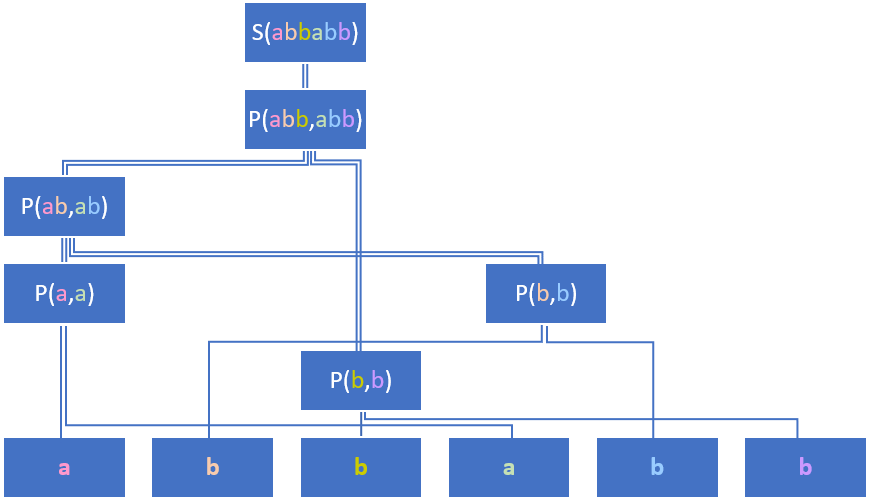
\includegraphics[width=\textwidth]{parse.png}
\caption{The parse tree for the string $abbabb$ using $G_{copy}$}
\label{fig:parse}
\end{figure}

Formally, an MCFG is defined as $(N,T,V,S,R)$, where:
\begin{itemize}
  \item $N$, $T$ and $V$
    are disjoint finite sets of non-terminal, terminal, and variable\linebreak symbols, correspondingly;
    for each $A\in N$, $dim(A)$ is a positive integer;
  \item $S\in N$  is the start symbol, and $\dim(S)=1$;
  \item $R$  is a finite set of rules of the form
    \begin{adjustwidth}{-2em}{0pt}\vspace{-2em}
      $$ A_0(Y_1,\ldots,Y_{\dim(A_0)}) \leftarrow A_1(X^{(1)}_1,\ldots,X^{(1)}_{\dim(A_1)}),\ldots,A_m(X^{(m)}_1,\ldots,X^{(m)}_{\dim(A_m)}) $$
    \end{adjustwidth}\vspace{-1em}
    ---where $A_i \in N$ for $0\leq i\leq m$, $X^{(i)}_j\in V$ for $1\leq i\leq m,\ 1\leq j\leq\dim(A_i)$,
    $Y_j\in \{T\cup V\}^+$ for $1\leq j\leq\dim(A_0)$,
    and additionally, denoting $Y_j$ as $y^{(1)}_j\ldots y^{(n_j)}_j$:
    \begin{adjustwidth}{-2.5em}{0pt}\vspace{-2em}
      $$ \{y^{(i)}_j\;|\;1\leq j\leq\dim(A_0),\ 1\leq i\leq n_j\}\cap V = \{X^{(i)}_j\;|\;1\leq i\leq m,\ 1\leq j\leq\dim(A_i)\} $$
      $$ X^{(i_1)}_{j_1} = X^{(i_2)}_{j_2}\ \longleftrightarrow\ i_1=i_2 \land j_1=j_2 $$
      $$ y^{(i_1)}_{j_1} = y^{(i_2)}_{j_2} \in V\ \longrightarrow\ i_1=i_2 \land j_1=j_2 $$
    \end{adjustwidth}
    These additional conditions mean that each variable must be used exactly once on each side of the rule:
    this is the ``linearity'' which the name of LCFRS refers to, and it means that each substring
    of the input string is used exactly once in constructing the internal nodes of the parse tree.
    Arguably, the ellipsis in NLs can be thought of as a non-linearity in the grammar:
    e.g., in \emph{Fred took a picture of you, and Susan of me}, both conjuncts include the same
    $[took\ a\ picture]_\textsc{vp}$ as the predicate.
\end{itemize}

The goal of this work was to automate finding an MCFG that is the best match for the given set of strings (\emph{corpus}).
This is the same goal as that of \cite{keinan}, whose work unfortunately hasn't demonstrated an ability
to learn a grammar that is appropriate for the given corpus.

\subsection{Related Works}

Learning a classic CFG from a given corpus had been attempted many times since the 1990s,
using such Machine Learning techniques as Genetic Algorithms (\cite{lankhorst}),
Simulated Annealing (\cite{katzir, keinan}),\linebreak
Recurrent Neural Networks with external stack memory (\cite{das})
and, more recently, without it (\cite{cartling}); and others. Yet, researchers haven't so far pursued
learning an MCFG, which is a more powerful and more expressive language formalization,
making the search space substantially larger.
\cite{avraham} used Simulated Annealing to infer certain properties of a Minimalist Grammar,
which is another formalization
framework going beyond the expressive power of CFGs; but he didn't aim to learn a whole grammar.

The novelty of this work includes both technical improvements,
allowing the learner to acquire a grammar more successfully than that of \cite{keinan},
-- and an analysis of
the learner's shortcomings that make it perform much better with some corpora than with others.


\section{Experimental setup}
\subsection{Fitness function}

The first decision in constructing a learner is to define what it means for a grammar to be
``the best match for the given corpus''. This work uses Minimum Description Length, introduced by \cite{rissanen},
as the cost function: a grammar describes the most regularities in the input data
if the binary encoding of the grammar, together with the binary encoding
of the input data using this grammar, takes up the fewest bits.
The two components of the MDL score are conventionally designated as $|G|$ and $|D:G|$ correspondingly.
All calculations allow fractional bit lengths, following the definition of entropy  by \cite{shannon}:
e.g.\ when the character set comprises five characters, then each character carries
$\log_2 5\approx2.3$ bits of information.

To calculate the MDL score, it is important exactly how the grammars and the data are encoded.
For MCFGs, the following encoding is used, which adds two special characters \texttt{\$} and \texttt{\#}
to the character set $N\cup T\cup V$: 
LHS uses \texttt{\$} as the separator and \texttt{\#} as the terminator;
RHS uses \texttt{\#} as the predicate terminator, and an additional \texttt{\#} as the rule terminator.
$G_{copy}$, specified in Figure \ref{fig:Gcopy}, is encoded into the following string: (line breaks added for clarity)
\begin{align*}
&\texttt{SXY\#PXY\#\#}\\
&\texttt{Pa\$a\#\#}\\
&\texttt{Pb\$b\#\#}\\
&\texttt{PXY\$ZW\#PXZ\#PYW\#\#}
\end{align*}

Now, there are restrictions on which characters may appear in each position:
the first character in each rule is a NT,
followed by a sequence of ``LHS characters'' out of $T\cup V\cup \{\texttt{\$}\}$, then a \texttt{\#};
thereafter, each NT is followed by a sequence of variable symbols, then a \texttt{\#}.
Therefore, each NT takes $\log_2(|N|+1)$ to encode, including the option for the rule terminator;
each LHS character takes $\log_2(|T|+|V|+2)$ to encode, including the option for the LHS terminator;
and each variable takes $\log_2(|V|+1)$ to encode, including the option for the predicate terminator.
The encoding of $G_{copy}$ includes 11 NT characters, each $\log_2 3\approx1.6$ bits long;
17 LHS characters, each 3 bits long; and 9 variable characters, each $\log_2 5\approx2.3$ bits long.
In total, $|G_{copy}|\approx74.7$ bits.

Encoding a string requires, for its derivation by means of the grammar,
specifying at each step which production is applied.
Thus, an NT with two alternative productions requires a single bit to encode; with three possible
productions, 1.6 bits; and if there's only one production possible, then no bits are necessary.
For example, the string $abab$ is derived as $S\rightarrow P\rightarrow PP \rightarrow aPa \rightarrow abab$ applying the sequence of rules (1), (4), (2), (3).
The first production is compulsory, and takes no bits to encode; each of the others takes 1.6 bits,
for a total of $|abab:G_{copy}|\approx4.8$ bits.
More generally, it can be seen that a string of length $2n$ takes $(2n-1)\log_2 3$ bits
to encode using $G_{copy}$.

To see how MDL favors the most ``meaningful'' grammar, consider the corpus consisting of the 40 strings
$\{aa, bb, aaaa, abab, baba, bbbb, aaaaaa, aabaab, \ldots\}$,
sampled from the aforementioned copy language. (The entire corpus is listed in the Appendix.) 
The total length of all input strings is 306 characters.
The target grammar $G_{copy}$ takes up 74.7 bits, and allows encoding the corpus in
$(306-40)\log_2 3\approx 421.6$ bits.
On the other hand, the trivial grammar $G_{con}$, shown in Figure \ref{fig:Gcon},
takes up only $11\log_2 3 + 9\log_2 6 + 6\log_2 3 \approx 50.2$ bits,
but then the corpus requires 612 bits to be encoded: each terminal symbol is encoded verbatim,
taking two bits, and making no use of the regularities in the input language.
$G_{con}$ allows encoding any string whatsoever, over-generalizing the input language to $\{a,b\}^+$.
Finally, the ``rote'' grammar, including a production rule for every string in the corpus:
\begin{align*}
&S(aa) \leftarrow\varepsilon \\
&S(bb) \leftarrow\varepsilon \\
&S(aaaa) \leftarrow\varepsilon \\
&S(abab) \leftarrow\varepsilon \\
&\ldots
\end{align*}
---allows encoding the corpus in just 212.9 bits (at $\log_2{40}\approx5.3$ bits per string),
but then the grammar's own encoding takes up $40\cdot2+(306+40)\cdot2 = 772$ bits.
$G_{rote}$ doesn't allow encoding any strings which aren't present in the input corpus -- in other words, it doesn't generalize the corpus to a bigger language.

\begin{figure}[t]
\begin{align*}
P(a) &\leftarrow\varepsilon \\
P(b) &\leftarrow\varepsilon \\
S(XY) &\leftarrow P(X),S(Y) \\
S(X) &\leftarrow P(X)
\end{align*}
\caption{The trivial grammar $G_{con}$ (for ``concatenation'')}
\label{fig:Gcon}
\end{figure}

To summarize:
\begin{table}[h]
\begin{tabular}{ c | c c c }
 grammar & $|G|$ & $|D:G|$ & MDL score \\ 
 \hline
 $G_{copy}$ & 74.7 & 421.6 & 496.3 \\  
 $G_{con}$ & 50.2 & 612.0 & 662.2 \\
 $G_{rote}$ & 772.0 & 212.9 & 984.9
\end{tabular}
\end{table}

$G_{copy}$ clearly wins over either encoding the input data verbatim,
or incorporating the whole corpus into the grammar.

To evaluate the MDL score for a grammar, it's necessary to parse every input string using the grammar.
This is done using a bottom-up Cocke--Younger--Kasami parser, adapted from \cite{kallmeyer}:
at each step, it tries to form new non-terminal nodes by combining nodes produced at the previous step
with those produced at all previous steps.
The parsing terminates when a node is produced for the start symbol $S$ and the whole input string.
This exhaustive-search strategy incurs a very high computational complexity, amounting to
$O(n^{d\cdot(r+1)})$, where $d$ is the dimension of the MCFG, i.e. the maximum dimension among all its NTs;
and $r$ is the rank of the MCFG, i.e. the longest concatenation on the LHS among all production rules.
In order to keep the parsing reasonably fast, the GA is disallowed to spawn MCFGs with $r>4$.

More specifically, a parser for \emph{probabilistic} MCFG is used, which, given the probability associated
with each production rule, finds the probability $P$ of the likeliest derivation for the input string:
then encoding the input string using the given grammar requires $(-\log_2{P})$ bits.
To be evaluated, an MCFG is first converted to a PMCFG for the parser by assigning, for each NT,
equal probabilities to all rules having the NT on the LHS.

\subsection{Search strategy}

The second important aspect of learning the best grammar is deciding on the strategy for finding it.
The search algorithm chosen for this work (Genetic Algorithm with multiple ``islands'')
may be summarized as follows:
\begin{itemize}
  \item Each island is initialized with the trivial grammar $G_{con}$, shown in Fig.\ \ref{fig:Gcon}.
  \item On each iteration, either one or two ``parents'' are chosen at random (non-uniformly),
    and a new grammar is spawned by combining the parents' rules,
    copying rules from the first parent up to a random point, then from the second parent (``crossover''),
    and/or by applying random small changes to the grammar (``mutations'').
  \item If the population of an island exceeds the limit, some of its grammars are killed at random
    (non-uniformly).
  \item Occasionally, each island sends a clone of one of its grammars to the next island,
    in a round-robin fashion, so that the local developments on each island
    are eventually shared with the rest of the population.
\end{itemize}
The probabilities of procreation, death, and migration are all determined by the grammar's relative rank
in the island's population, rated by the MDL score.


\subsection{Implementation}

The learner is implemented in Python, and split into four modules:
\begin{itemize}
  \item \texttt{Grammar.py} implements the object model for PMCFG (classes \texttt{Pred, PRule, Grammar}),
    the latter including the ruleset for grammar mutations;
  \item \texttt{Parser.py} implements a CYK parser for PMCFG, adapted from \cite{keinan}:
    some technical improvements to his code, e.g. using Python frozen data classes,
    allowed to speed up parsing by an order of magnitude, while retaining the same essential algorithm;
  \item \texttt{GeneticAlgorithm.py} implements the GA for finding the best MCFG, including
    MDL scoring and a simple visualization of the evolution progress,
    relying on the \texttt{graphics} library for Python by \cite{zelle};
  \item \texttt{Main.py} sets the input corpus, initial grammar, and other meta-parameters for the GA.
\end{itemize}

A technical limitation of the PMCFG parser being used is that terminal symbols can only appear
with unary NTs, on the LHS of trivial terminal rules of the form $N(t)\leftarrow\varepsilon$.
This restriction, reminiscent of the Chomsky normal form for CFGs (\cite{chomsky1959}),
doesn't affect the expressive power of MCFGs, as any MCFG can be normalized into such a form;
moreover, for grammars used in NLP, such form is most natural, as each terminal symbol
(corresponding to a lexicon entry) is first categorized as a part of speech,
before being used in further productions.

On the other hand, the parser being used is less restrictive than the formal definition of (P)MCFG
as given in the Introduction,
in that it doesn't require every variable predicated on the RHS of a production rule to be used on its LHS.
E.g., the rule $S(X) \leftarrow P(X)R(Y)$ means ``$S$ can be produced from $P$ if $R$ can be produced
from any substring of the input string'', and $S(X) \leftarrow P(X,Y)$ means ``$S$ can be produced from
a substring if $P$ can be produced from it and some other substring of the input string'' --
similar to the lookahead/lookbehind features of extended regular expressions.
It was shown by \cite{kallmeyer} that the requirement for all predicated variables to be used on the LHS
doesn't affect the expressive power of MCFG; for the purposes of GA, it is helpful
that mutation chains are allowed to include intermediate grammars whose rules include unused variables.

An important part of designing the GA was to define the ruleset for mutations, making sure that
all mutations result in valid MCFGs, and every valid MCFG can be reached via a chain of mutations.
The following 15 rules are used:
\begin{enumerate}[itemsep=-2.3pt]
  \item Add a new terminating rule for an existing or a new NT;
  \item Add an aliasing rule between two NTs of the same dimension;
  \item Add a concatenating rule with two unary NTs on the RHS;
  \item Delete a random rule;
  \item Expand a unary NT using a random production rule;
  \item Add a random NT on the RHS, ignore its predicated variables on the LHS;
  \item Delete a NT whose predicated variables are ignored on the LHS;
  \item Delete the use of a random variable on the LHS;
  \item Concatenate an unused variable in a random position on the LHS;
  \item Split a NT, adding a new dimension, e.g. $P(XY) \leftarrow A(X)B(Y),\ S(X) \leftarrow P(X)$ into $P(X, Y) \leftarrow A(X)B(Y),\ S(XY) \leftarrow P(X, Y)$;
  \item Merge two dimensions of a NT (i.e. the inverse of the above);
  \item Swap two dimensions of a multidimensional NT on the LHS;
  \item Swap two variables in a concatenation on the LHS;
  \item Mutate the terminal symbol in a terminal rule;
  \item Mutate a NT symbol on either side of a rule.
\end{enumerate}

\section{Experimental results}
The settings used for the GA in the experiments were as follows: 10,000 iterations;
10 islands of up to 200 grammars each;
mortality rate 50\% for the lowest scored grammar, decreasing exponentially with the rank;
mutation rate 60\%; crossover rate 20\%; and migrations every 100 iterations.
If a grammar fails to produce some of the words in the training set,
its $|D:G|$ score receives a penalty of 35 bits for each such word.
Before calculating $|G|$, each grammar is stripped of all non-reachable rules and NTs,
and the penalty for having them is $(|G_{original}|-|G_{stripped}|)/100$ --
in most observed cases, the penalty amounts to a few tenths of a bit.
This allows ``dormant'' rules, facilitating multi-stage improvement,
to remain in the best-performing grammars, while still applying a slight pressure to get rid of them.

Figure \ref{fig:progress} illustrates the evolution of the grammars:
each of the 10 graphs corresponds to an island, the green line is the best score in the population,
the red is the worst, and the brown is the average. Each horizontal pixel is one generation,
for a total of 1800$\times$10 generations, and each vertical pixel is 50 score points.
During the first 200 generations, no grammars die, and the average score gradually worsens.
Then, over a few hundred generations, bad grammars die out, and the average score gradually improves.
After such a ``ramp-up'', the average score approaches the best, and the worst shows
increasingly erratic fluctuations corresponding to newly spawned bad grammars staying alive
for up to a dozen or two generations.

\begin{figure}[b!]
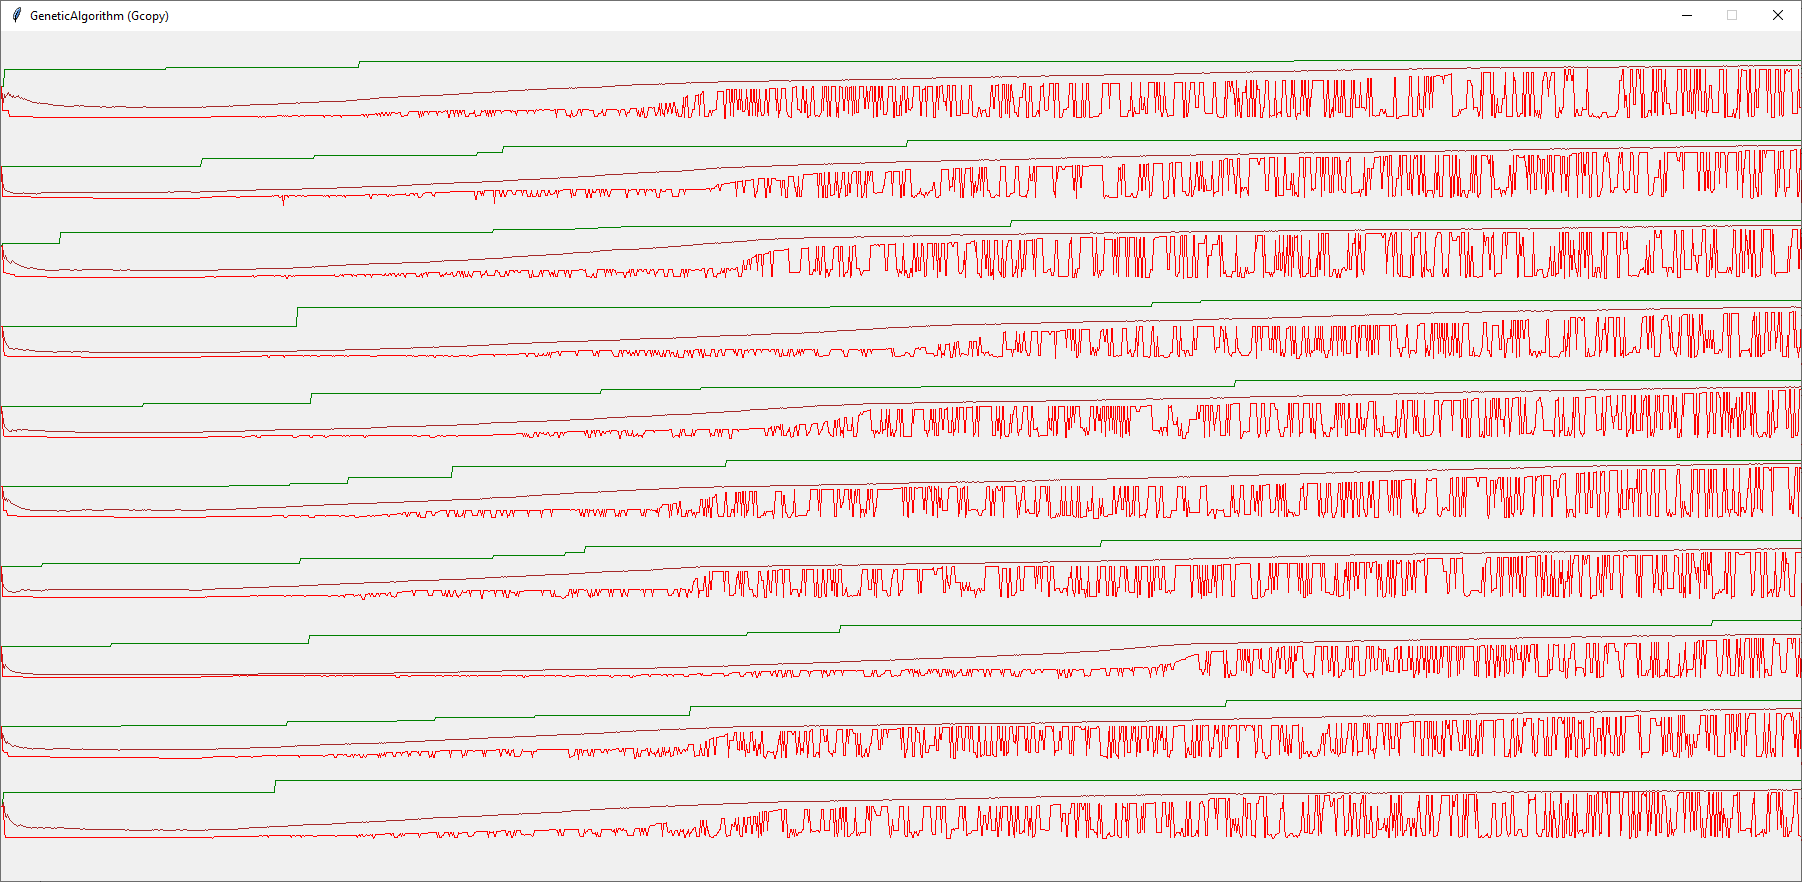
\includegraphics[width=\textwidth]{progress.png}
\caption{Evolution targeting $G_{copy}$}
\label{fig:progress}
\end{figure}

The GA took 4,088 iterations to arrive at a grammar equivalent to the following CFG,
which will be referred to as $G_{opt}$:
\begin{align*}
A &\rightarrow a\,|\,b \\
S &\rightarrow AA\,|\,ASA
\end{align*}

$G_{opt}$ expresses only the generalization that all input strings have even length.
Unexpectedly, $|G_{opt}|=71.1$ and $|D:G_{opt}|=459$, so that the resulting MDL score of 530.1 bits
beats the target $G_{copy}$ by a small margin. The reason is that its savings on being very simple
outweigh its losses on over-generalizing the input language.
In order to account for this, the score calculation has been changed from pure MDL to
$|G| + 3\times|D:G|$, as if the corpus had three copies of each input string,
so that the over-generalization incurs three times the loss.
This way, the target grammar's score remains lower than that of the distractor:

\begin{table}[h]
\begin{tabular}{ c | c c c c }
 grammar & $|G|$ & $|D:G|$ & $|G| + |D:G|$ & $|G| + 3\times|D:G|$ \\ 
 \hline
 $G_{con}$ (initial) & 48.6 & 612.0 & 660.6 & 1884.6 \\
 $G_{opt}$ (result) & 71.1 & 459.0 & 530.1 & 1448.1 \\  
 $G_{copy}$ (target) & 144.3 & 421.6 & 565.9 & 1409.1
\end{tabular}
\end{table}

Even with the updated scoring, the best found grammar $G_{opt'}$ remained weakly-equivalent to $G_{opt}$,
describing the same effective language $(a|b)^{2n}$ -- but $G_{opt'}$ allows shallower derivations
than $G_{opt}$, thus lowering the description length for longer input strings at the expense of shorter ones:
\begin{align*}
A &\rightarrow PP\\
P &\rightarrow a\,|\,b\\
C &\rightarrow A\,|\,AA\\
S &\rightarrow C\,|\,ASA
\end{align*}

$|G_{opt'}|=135.7$ and $|D:G_{opt'}|=434$, therefore its score 1437.7 is still above the target.
Yet, the target grammar --
in fact, any MCFG making use of multidimensional NTs and thereby transcending the expressive power
of classic CFGs -- wasn't reached during the experiment, which took a couple of days to run on my laptop.

To assess whether the failure is due to peculiarities of the specific target language,
or the search space of MCFGs in general, or the implementation and settings of the GA, --
experiments were run, using the same settings, with three other corpora,
sampled from the language of palindromes $\{a, b, aa, bb, aaa, aba,\\ bab, \ldots\}$
(27 strings in total),
and from two powers languages, $\{ab, aabb, aaabbb,\\ aaaabbbb, aaaaabbbbb\}$ and
$\{abc, aabbcc, aaabbbccc, aaaabbbbcccc\}$.


\section{Discussion}

To see why $G_{copy}$ hadn't been reached, I've manually constructed two mutation chains,
shown in Figure \ref{fig:chains}: each column shows the two components of the MDL score
for an intermediate grammar along the chain.
(To make variations in both $|G|$ and $|D:G|$ discernible, the scores are plotted on a logarithmic scale.)
These two chains are certainly not the only ones possible, and they may not be the shortest either;
but they do illustrate the difference in ``steepness'' between the two transitions:
in the chain $G_{con} \rightarrow G_{opt}$, the longest ``uphill walk'' is two steps, incurring a 12\% increase in score;
whereas in $G_{opt} \rightarrow G_{copy}$, it is six steps, incurring a $\times$2.7 increase.
It seems natural that the latter chain is too steep for the GA to climb.

\begin{figure}[t]\centering
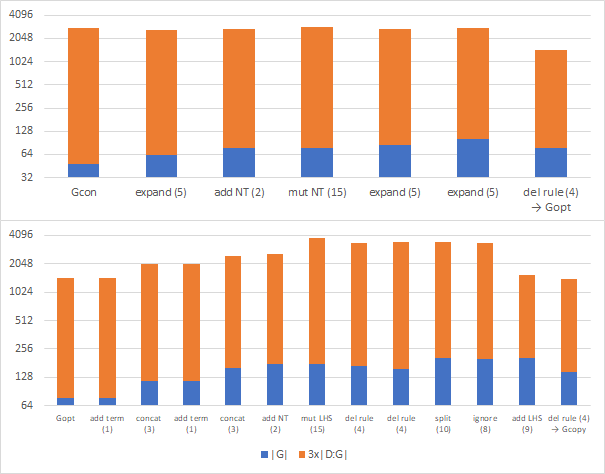
\includegraphics[width=.85\textwidth]{chains.png}
\caption{Mutation chains $G_{con} \rightarrow G_{opt}$ and $G_{opt} \rightarrow G_{copy}$}
\label{fig:chains}
\end{figure}

The results for the three other corpora have been somewhat more successful: it is noteworthy that
the very small samples from the powers languages didn't lead to emergence of ``rote'' grammars.
\begin{itemize}
  \item For the language $a^n b^n$, the learner easily found the target grammar $G_{a^n b^n}$,
    equivalent to the CFG $A\rightarrow a,\ B\rightarrow b,\ S\rightarrow AB\,|\,ASB$:
    
    \begin{tabular}{ c | c c c c }
     grammar & $|G|$ & $|D:G|$ & $|G| + |D:G|$ & $|G| + 3\times|D:G|$ \\ 
     \hline
     $G_{con}$ (initial) & 48.6 & 60.0 & 108.6 & 228.6 \\
     $G_{a^n b^n}$ (target) & 74.9 & 15.0 & 89.9 & 119.9
    \end{tabular}\vspace{1ex}

  \item For the language $a^n b^n c^n$, the best grammar $G_{result}$ found by the learner
    was equivalent to the following CFG:
    \begin{align*}
    A &\rightarrow a\\
    B &\rightarrow b\\
    C &\rightarrow c\\
    P &\rightarrow PB\,|\,C\\
    S &\rightarrow ASP\,|\,b
    \end{align*}
    ---whose effective language is $a^n b (b^{*}c)^n$.
    The initial grammar $G_{con'}$ was different from the other experiments in that it allowed
    three terminal characters $\{a,b,c\}$. The target MCFG $G_{a^n b^n c^n}$:
    \begin{align*}
    A(a) &\leftarrow\varepsilon\\
    B(b) &\leftarrow\varepsilon\\
    C(c) &\leftarrow\varepsilon\\
    P(X,Y,Z) &\leftarrow A(X),B(Y),C(Z)\\
    P(XU,YV,ZW) &\leftarrow A(X),B(Y),C(Z),P(U,V,W)\\
    S(XYZ) &\leftarrow P(X,Y,Z)
    \end{align*}
    ---was not found. This time, the target grammar is so complex that even the 3$\times$ factor
    wasn't enough to bring its MDL score below that of $G_{result}$:

    \vspace{1ex}\begin{tabular}{ c | c c c c }
     grammar & $|G|$ & $|D:G|$ & $|G| + |D:G|$ & $|G| + 3\times|D:G|$ \\ 
     \hline
     $G_{con'}$ (initial) & 59.4 & 112.0 & 171.4 & 395.4 \\
     $G_{result}$ & 100.5 & 30.0 & 130.5 & 190.5 \\
     $G_{a^n b^n c^n}$ (target) & 192.9 & 10.0 & 202.9 & 222.9
    \end{tabular}\vspace{1ex}
  
  \item Last, for the language of palindromes, the target grammar equivalent to the CFG
    \begin{align*}
    A &\rightarrow a\\
    B &\rightarrow b\\
    S &\rightarrow ASA\,|\,BSB\,|\,AA\,|\,BB\,|\,a\,|\,b
    \end{align*}
    ---was not found; instead, the learner optimized the initial grammar $G_{con}$ into $G_{opt''}$
    which is equivalent to the CFG 
    \begin{align*}
    P &\rightarrow a\,|\,b\\
    C &\rightarrow P\,|\,PP\\
    S &\rightarrow C\,|\,PSP
    \end{align*}
    ---and allows shallower derivations than $G_{con}$ while describing the same effective language
    $\{a,b\}^{+}$. This case, same as for the copy language, may be considered the learner's failure,
    as the target grammar has lower MDL score than that of the found grammar:

    \begin{tabular}{ c | c c c c }
     grammar & $|G|$ & $|D:G|$ & $|G| + |D:G|$ & $|G| + 3\times|D:G|$ \\ 
     \hline
     $G_{con}$ (initial) & 48.6 & 264.0 & 312.6 & 840.6 \\
     $G_{opt''}$ (result) & 106.1 & 233.0 & 339.1 & 805.1 \\  
     $G_{pal}$ (target) & 151.8 & 191.3 & 343.0 & 725.6
    \end{tabular}
\end{itemize}

To conclude, we may estimate that
MCFGs present difficulties for GA because of the non-local constraints on a grammar's validity:
e.g. all appearances of a NT must have the same dimension, the two sides of a production rule
must have the same variables without omissions or repetitions, etc.
As a result, the mutation rules have to be quite complex: e.g. the split rule (\#10) involves
updating all productions where the NT appears on either side. On the other hand,
classic CFGs, where any string of grammar symbols is a valid RHS for any production, are trivial to mutate;
and so, small mutations tend to cause small changes to the grammar's performance.
As the GA in the experiments has never found multidimensional NTs useful,
effectively it was searching in the subspace of classic CFGs, but using the MCFG mutation rules. 


\section{Further work}

Possible improvement of the learner may follow these two directions: the first is to use, instead of MCFG,
an equally expressive formalism
whose representation of a grammar may have less internal structure, making it more amenable to mutations.
Minimalist Grammars, used by \cite{avraham}, may (or may not) be such an option.
The other direction, \emph{a priori} seeming more promising,
is to find a robust way of choosing the meta-parameters for the GA,
such as population sizes, mutation rates, longevity of individual grammars, etc.
For the experiments described in this work, all meta-parameters values were picked based on intuition
alone, and their effect had not been rigorously evaluated;
the only observation has been that slight changes don't have any noticeable effect.


\section*{Appendix: Code and input data}

The code of the learner is available on GitHub: \url{https://github.com/tyomitch/pmcfg};
for visualization, it uses the \texttt{graphics} library by \cite{zelle},
available at \url{https://mcsp.wartburg.edu/zelle/python/graphics.py}

The following 40 strings comprise the corpus for the copy language:\\
$\{aa,bb,aaaa,abab,baba,bbbb,aaaaaa,aabaab,abaaba,baabaa,abbabb,bbabba,\\
bbbbbb,aaaaaaaa,aaabaaab,aabaaaba,abaaabaa,baaabaaa,aabbaabb,abbaabba,\\
bbaabbaa,abbbabbb,bbbabbba,abababab,babababa,bbbbbbbb,aaaaaaaaaa,\\
aaaabaaaab,aaabaaaaba,aabaaaabaa,abaaaabaaa,baaaabaaaa,aaabbaaabb,\\
aabbaaabba,abbaaabbaa,bbaaabbaaa,aabbbaabbb,abbbaabbba,bbbaabbbaa,\\
abbbbabbbb\}$

The following 27 strings comprise the corpus for the language of palindromes:\\
$\{a,b,aa,bb,aaa,aba,bab,bbb,aaaa,abba,baab,bbbb,aabaa,baaab,abbba,abaaba,\\ abbabba,abbaabba,abababa,aabaaabaa,babab,babbab,abaaaba,aaabaaa,aabbbaa,\\
abbbba, babbbbab\}$

The corpora used for the two powers languages are $\{ab, aabb, aaabbb, aaaabbbb,\\ aaaaabbbbb\}$ and $\{abc, aabbcc, aaabbbccc, aaaabbbbcccc\}$.


\bibliographystyle{authordate1}
\bibliography{references}
\end{document}
